\documentclass[11pt]{article}
\usepackage{amsmath,amssymb,amsthm}
\usepackage{enumitem}
\setlist{itemsep=0pt}
\usepackage{tikz} 
\usetikzlibrary{calc, shapes, matrix, arrows}
\tikzset{>=latex}

\DeclareMathOperator*{\E}{\mathbb{E}}
\let\Pr\relax
\DeclareMathOperator*{\Pr}{\mathbb{P}}
\mathchardef\mhyphen="2D

\newcommand{\eps}{\varepsilon}
\newcommand{\inprod}[1]{\left\langle #1 \right\rangle}
\newcommand{\R}{\mathbb{R}}

\newcommand{\handout}[5]{
  \noindent
  \begin{center}
  \framebox{
    \vbox{
      \hbox to 5.78in { {\bf CS 224: Advanced Algorithms } \hfill #2 }
      \vspace{4mm}
      \hbox to 5.78in { {\Large \hfill #5  \hfill} }
      \vspace{2mm}
      \hbox to 5.78in { {\em #3 \hfill #4} }
    }
  }
  \end{center}
  \vspace*{4mm}
}

\newcommand{\lecture}[4]{\handout{#1}{#2}{#3}{Scribe: #4}{Lecture #1}}

\newtheorem{theorem}{Theorem}
\newtheorem*{corollary}{Corollary}
\newtheorem{lemma}{Lemma}[section]
\newtheorem{observation}{Observation}
\newtheorem*{example}{Example}
\newtheorem{proposition}[theorem]{Proposition}
\newtheorem*{definition}{Definition}
\newtheorem*{claim}{Claim}
\newtheorem{fact}[theorem]{Fact}
\newtheorem{assumption}[theorem]{Assumption}

% 1-inch margins, from fullpage.sty by H.Partl, Version 2, Dec. 15, 1988.
\topmargin 0pt
\advance \topmargin by -\headheight
\advance \topmargin by -\headsep
\textheight 8.9in
\oddsidemargin 0pt
\evensidemargin \oddsidemargin
\marginparwidth 0.5in
\textwidth 6.5in

%\parindent 0in
%\parskip 1.5ex

\begin{document}

\lecture{25 --- April 18, 2017}{Spring 2017}{Prof.\ Jelani Nelson}{Christina Chen (w/ Nithin Tumma Fall'14 notes on scaling)}

\section{Overview}

In the last lecture, we analyzed Ford-Fulkerson. In this lecture, we consider two ways to find max flows more quickly than Ford-Fulkerson.

\section{Scaling Capacities}
Recall that the Ford-Fulkerson algorithm has runtime $O(mf^*)$, where $f^*$ is the maximum flow. We want to improve on the factor of $f^*$. The idea is to think of each capacity $c (e)\in \{1, 2 \ldots U\}$  as a bit integer $u(e) \in \{0, 1\}^{\lceil \log_2 U \rceil}$. Then, we will ``process'' each $u(e)$ one bit at a time (from left to right), maintaining capacities $u'(e) = u(e)_{n \ldots (n-k)}$ (th $k$ most significant bits of $u$) and a flow $f'$ such that $f'$ is feasible on $u'(e)$. We will actually ensure that $f'$ is optimal at the beginning of each iteration. Then, when we finish, $u'(e) = u(e)$ and we will have $f' = f^*$. The complete scaling algorithm is given below. This algorithm is due to Gabow \cite{Gabow}. 

\subsection{Scaling Max-Flow Algorithm}
\begin{itemize}
\item initialize  $u'(e) = 0, f'_e = 0$ for all $e \in E$. 
\item for $k = (\lceil \log_2 U \rceil - 1) \ldots 0$
	 \begin{itemize}
 		\item for each $e \in E$ 
			\begin{itemize}
				\item set $u'(e) = 2u'(e)$ and $f'_e = 2f'_e$ (add trailing 0 to bit vectors of $u', f'$)
			\end{itemize} 
		\item for each $e \in E$ 
			\begin{itemize}
				\item set $u'(e) = u'(e) + u(e)_k$  (add $k$'th bit of $u$ to $u'$)
			\end{itemize} 
		\item augment $f'$ such that it is a max flow for $G$ with capacities $u'(e)$ 
 	\end{itemize}
\end{itemize}

\subsection{Analysis}
\begin{claim}
At the beginning of every iteration of the scaling algorithm, $f' = (f')^*$, the maximum flow on $G$ with capacities $u'(e)$. 
\end{claim}
\begin{proof}
At the beginning of the first iteration $u'(e) = 0  ~ \forall e \in E$ so $(f')^* = 0 = f'$. Now, suppose that $f' = (f')^*$ before we update $u'(e)$. Then, there must exist some saturated $S-T$ cut in $(G, u')$. After we double $u'(e)$ and $f'_e$, the cut is still saturated. After we add $u(e)_k$ to $u'$, $f'$ may not be maximal, but it is still feasible. But then we augment $f'$ so that it must equal $(f')^*$ on the new capacities. 
\end{proof}

% maybe make the proof of correctness a claim?
At the $k$'th iteration of the algorithm $u'(e)$ is the $k$ most significant bits of $u(e)$, so after $\lceil \log_2 U \rceil $ iterations $u'(e) = u(e)$. Hence, by the claim, the output $f'$ of the scaling algorithm will be the maximal flow for $G$ with capacities $u'(e) = u(e)$, as desired. 

The scaling algorithm runs for $O(\log_2 U)$ iterations, each iteration dominated by the time to augment $f'$ into a maximal flow. If we use Ford-Fulkerson, we know that this time will be $O(m f^*)$. What can we say about $f^*$? 

\begin{claim}
In each iteration of the scaling algorithm, $f' = f^* \leq m$. 
\end{claim}

\begin{proof}
At the beginning to the current iteration $f' = (f')^*$, so there must exist some saturated $S-T$ cut of $(G, u')$. Now, as before, after we double $u'(e), f_e'$, this cut will still have 0 capacity. After we set $u'(e) = u(e)_k$, we can have increased $u'(e)$ by at most $1$. Since the cut cannot contain more than $m$ edges, its residual capacity is $\leq m$ now, so the minimum cut in $(G, u')$ must have capacity $\leq m$ which implies that $f^* \leq m$ (by the max-flow min-cut theorem). 
\end{proof}

Hence, if we use Ford-Fulkerson to augment $f'$, each iteration takes $O(m + m f^*) = O(m^2)$ steps, so we can achieve a runtime of $O(m^2\log U)$ for maximum flow using the scaling algorithm. Hence, the scaling algorithm is weakly polynomial. 

\section{Blocking Flow}
Suppose we have a residual graph $G_f$. For any $v\in V$, let its \textbf{level} $\ell_v$ denote the length of the shortest path distance from $s$ to $v$ in $G_f$.

\begin{definition}
An edge $(u,\, v)\in E$ is \textbf{admissible} if $\ell_v=\ell_u+1$. An $s\mhyphen t$ flow on $G_f$ is \textbf{admissible} if it traverses only admissible edges.
\end{definition}
\begin{definition}
The \textbf{level graph} $L$ associated with $G_f$ is the subgraph of $G_f$ comprising only its admissible edges.
\end{definition}
\begin{definition}
A \textbf{blocking flow} $f$ is an admissible $s\mhyphen t$ flow that saturates at least one edge in every other admissible flow $f'$.
\end{definition}

\begin{example}
Consider the following unit-capacity residual graph. 
$$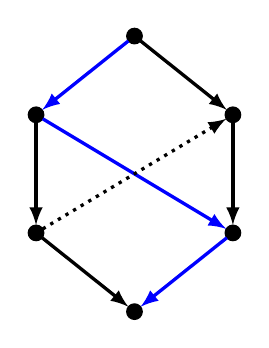
\begin{tikzpicture}[every node/.style={draw,shape=circle,inner sep=2pt,outer sep=0pt, fill=black}]
\path (0,0) node (p0) {}
(-1.25,-1) node (p1) {}
(-1.25,-2.5) node (p2) {}
(1.25,-2.5) node (p3) {}
(1.25,-1) node (p4) {}
(0,-3.5) node (p5) { };
\draw[->,blue, very thick](p0)--(p1);
\draw[->, very thick](p1)--(p2);
\draw[->, very thick](p0)--(p4);
\draw[->, very thick](p4)--(p3);
\draw[->, very thick](p2)--(p5);
\draw[->, blue, very thick](p3)--(p5);
\draw[->, blue, very thick](p1)--(p3);
\draw[->, dotted, very thick](p2)--(p4);
\end{tikzpicture}$$
The blue flow is a blocking flow but clearly not a max flow. On the other hand, by definition, every admissible max flow is a blocking flow. Moreover, all edges here except for the dotted one are in the associated level graph.
\end{example}

\subsection{A new algorithm for max flow}
Recall that one of the shortcomings of Ford-Fulkerson is that the algorithm can run up to $f^*$ iterations. We will see how blocking flows remedy this problem.

\begin{lemma}\label{increased}
Augmenting along a blocking flow strictly increases $d(s,\, t)$  in the new level graph.
\end{lemma}
\begin{proof}
Let $L'$ denote the level graph after augmenting along a blocking flow. Since we augmented along a flow in $L$, it is clear that $$L'\subseteq L\cup\text{rev}(L)\cup (G_f\backslash L),$$ where $\text{rev}(L)$ denotes the set comprising the edges in $L$ reversed. But this implies that $d_{\scriptscriptstyle L'}(s,\, t)\geq d_{\scriptscriptstyle L}(s,\, t)$. However, if $d_{\scriptscriptstyle L'}(s,\, t)=d_{\scriptscriptstyle L}(s,\, t)$, then $L$ and $L'$ must share some $s\mhyphen t$ path, which contradicts the fact that we constructed $L'$ from $L$ by augmenting along a blocking flow.
\end{proof}

Why is this useful? Consider the following algorithm, given by Dinitz in \cite{Dinitz}. 
\begin{enumerate}
\item Initialize $f$ to 0.
\item While there exists an $s\mhyphen t$ path in $G_f$, augment $f$ along a blocking flow.
\end{enumerate}

It is clear that when we terminate the process, we have found a max flow. 

\begin{observation}\label{runtime}
Dinitz's runtime is given by $(\#\text{ iterations})\times(\text{time to find blocking flow})$.
\end{observation} 
Lemma~\ref{increased} implies that the first term is at most $n-1$. We will consider the second term below. 

\subsection{Finding a blocking flow}\label{findflow}
We do so by running a modified version of DFS on $L$ from $s$ to build a blocking flow $f\in\mathbb{R}^m$. 

We initialize $f$ to 0 and $H$ to $L$. From our current vertex $v$, we may run three kinds of moves.
\begin{itemize}
\item $\text{advance}(v,\, w)$: move from $v$ to $w$ for $(v,\, w)\in L$,
\item $\text{retreat}(u,\, v)$: if $\nexists$ $(v,\, w)\in L$, return its ancestor $u$ in the call stack and delete $(u,\, v)$ from $H$,
\item $\text{augment}$: if $v=t$, augment $f$ along the minimum residual flow on the found $s\mhyphen t$ path and delete saturated edges.
\end{itemize}

\subsubsection{Runtime analysis}
\begin{claim}
In unit capacity graphs, Section~\ref{findflow}'s algorithm considers each edge $O(1)$ times, which implies $O(m)$ time to find a blocking flow.
\end{claim}
\begin{proof}
Observe that the algorithm 
\begin{itemize}
\item advances at most once along any edge because $L$ is a DAG by construction,
\item retreats at most once along any edge because we delete it afterwards,
\item augments at most once along any edge because one augmentation immediately saturates it.
\end{itemize} It follows that the algorithm processes each edge only a constant number of times.
\end{proof}

Then Observation~\ref{runtime} implies the following.
\begin{corollary}
In unit-capacity graphs, Dinitz's algorithm runs in $O(mn)$ time.
\end{corollary}

Note that in unit-capacity graphs, the cut crossing the edges from $s$ encounters at most $n-1$ units of flow. Then min-cut implies that $f^*\leq n-1$, so Ford-Fulkerson runs in $O(mn)$ time. 

It seems like our new algorithm exhibits no improvement. But it turns out that it guarantees better performance on unit-capacity graphs.

\begin{claim}
In unit-capacity graphs, Dinitz's algorithm runs $O(\min\{\sqrt{m},\, n^{2/3}\})$ iterations of finding blocking flows.
\end{claim}
\begin{proof}
$\mathbf{\sqrt{m}}$\textbf{-bound.}
\noindent Lemma~\ref{increased} implies that $d(s,\, t)\geq k$ after $k$ iterations of finding blocking flows. Unit capacity implies that any $s\mhyphen t$ flow can be decomposed into an edge-disjoint collection of $s\mhyphen t$ paths, so at most $\frac{m}{k}$ $s\mhyphen t$ path remain. Therefore, the residual max flow (equivalently, the number of iterations) is at most $\frac{m}{k}$. This means that the total number of iterations is at most $k+\frac{m}{k}$, which equals $2\sqrt{m}$ when $k=\sqrt{m}$.

$\mathbf{n^{2/3}}$\textbf{-bound.} 
In $L$, define $D_i:=\{v\in V:\ell_v=i\}$. Suppose that we have already run $k\geq 2n^{2/3}$ iterations, so $0\leq i\leq k$. Since at most half of the $D_i$ contain at least $n^{1/3}$ vertices, it follows that there must exist consecutive sets $D_i,\, D_{i+1}$ such that both contain at most $n^{1/3}$ vertices. Therefore, the number of edges from $D_i$ to $D_{i+1}$ is at most $|D_i|\cdot|D_{i+1}|\leq n^{2/3}$. This means that the cut crossing these edges encounters at most $n^{2/3}$ units of flow. Then min-cut implies that the remaining flow is at most $n^{2/3}$, so we run at most $2n^{2/3}+n^{2/3}=O(n^{2/3})$ iterations in total. 
\end{proof}

\begin{corollary}
In unit-capacity graphs, Dinitz's algorithm runs in $O(m\min\{\sqrt{m},\, n^{2/3}\})$ time.
\end{corollary}

\subsection{General capacity graphs}
We run the same algorithm, although the runtime now differs. 

\begin{itemize}
\item We retreat at most once along each edge, so retreats contribute $O(m)$ time. 
\item We saturate at least one edge each time we augment, so we augment at most $m$ times. The length of an $s\mhyphen t$ path is at most $n$, so augmentations contribute $O(mn)$ time. \item We can advance at most $n$ times before retreating, so advances contribute $O(mn)$ time. 
\end{itemize} 

This implies the following.

\begin{claim}
In general-capacity graphs, Dinitz's runs $O(mn)$ iterations of finding blocking flows.
\end{claim}
\begin{corollary}
In general-capacity graphs, Dinitz's runs in $O(mn^2)$ time.
\end{corollary}

It is also possible to show the in general capacity graphs, Dinitz' algorithm has runtime $O(mn + nf^*)$. Then since $f^*$ in each round of scaling is at most $m$ (since the previously saturated minimum cut now has at most $m$ units of added capacity), each round of scaling when using Dinitz' algorithm would take $O(mn)$ time. Thus using the capacity-scaling approach with Dinitz' algorithm used in each iteration would yield an overall runtime of $O(mn\log U)$.


\bibliographystyle{alpha}

\begin{thebibliography}{42}

\bibitem{Dinitz}
Yefim~Dinitz.
\newblock Algorithm for solution of a problem of maximum flow in a network with power estimation.
\newblock {\em Dokl. Akad. Nauk SSSR}, 11(5):1277--1280, 1970.

\bibitem{Gabow}
Harold~N.~Gabow.
\newblock Scaling Algorithms for Network Problems.
\newblock {\em J. Comput. Syst. Sci.} 31(2), pages 148--168, 1985.

\end{thebibliography}

\end{document}